
\section{Introduction}

\begin{figure}[t]
    \centering
    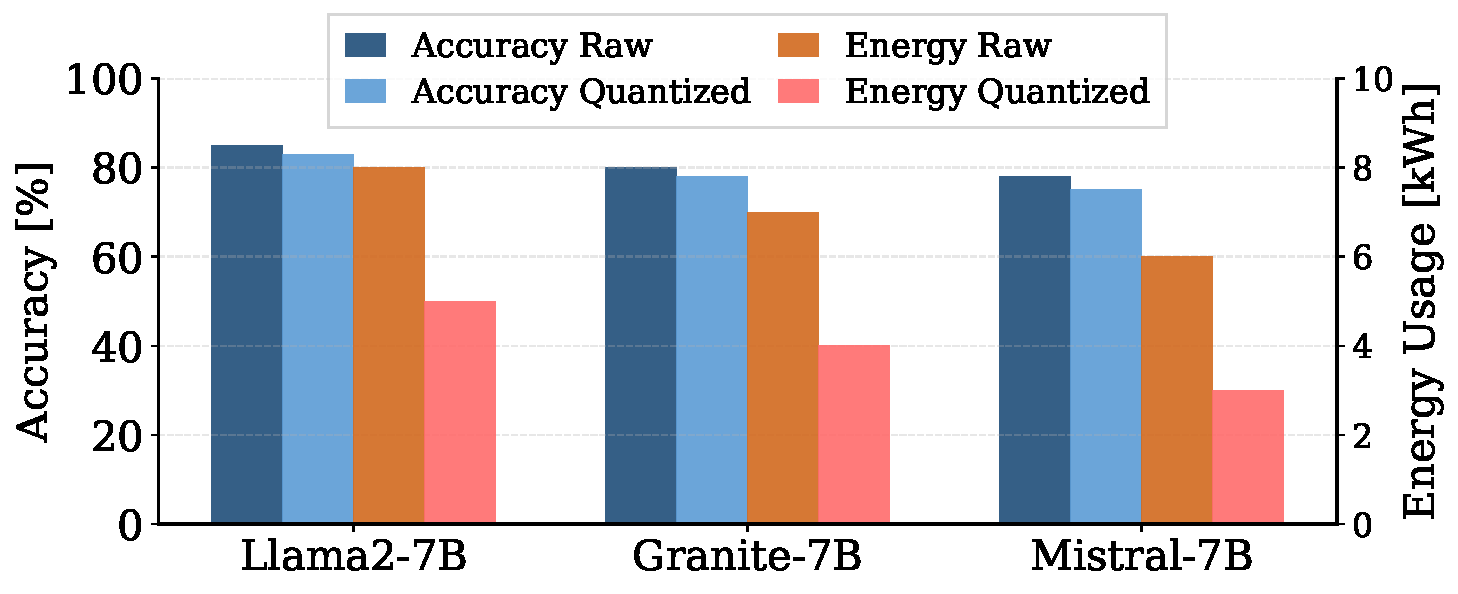
\includegraphics[width=0.95\linewidth]{reportTemplate/figures/f1.pdf}
    \caption{Mock! \underline{Quanti}fying the accuracy of LLMs, and energy consumption of LLMs under workload, compressed by quantization, uncompressed, and contrasted by architecture. Experimental methodology and details available in §\ref{sec:experiments}.}
    \label{fig:f1}
    
\end{figure}

% \lipsum[1-7]
Large Language Models (LLMs) have been used in a large number of applications of artificial intelligence recently, particularly in software engineering and natural language processing~\cite{DBLP:journals/corr/abs-1910-01108, 10968787}. However, these models are often so large that they contain billions of parameters ultimately creating significant sustainability challenges when used on a massive scale~\cite{DBLP:journals/tacl/ZhuLLMW24, DBLP:journals/corr/abs-1910-01108}. The trend of using LLMs in applications is on the rise, resulting in exponentially scaling computational requirements and substantial environmental costs. For example, one research shows that 16.68 tons of CO2 are emitted just by training a model called StarCoder, with 7 billion parameters~\cite{DBLP:journals/corr/abs-2507-09665}. While training is a considerable expense, a large number of environmental and computational costs typically rise after deployment, with inference energy consumption often bypassing training over time \cite{DBLP:journals/corr/abs-2507-09665}. These rising demands also put substantial memory and processing burdens, which slow down the widespread adoption of LLMs in real-time applications \cite{DBLP:journals/corr/abs-1910-01108}.



To tackle these challenges, researchers have explored several compression techniques to improve the performance, efficiency, and overall sustainability of LLMs. Although it is important to make LLMs more manageable, LLM comparison can introduce inherent tradeoffs, most notably a potential reduction in accuracy because of such compression methods. Among these is a compression technique known as quantization, which is used to decrease the parameter precision (e.g., from 32-bit floating point to 8-bit or 4-bit integers), which reduces the model size and computational demands without affecting the performance significantly or requiring any extensive retraining \cite{DBLP:journals/corr/abs-2507-09665, 10968787}. To reduce the demands for LLM resources, the CO2 footprint and energy consumption, quantization has been chosen as a reliable choice \cite{DBLP:journals/corr/abs-2507-09665}. Empirical evidence shows that quantization can lead to reductions in energy consumption and CO2 emissions up to 45\% after quantification \cite{DBLP:journals/corr/abs-2504-06307}. It can also reduce the memory utilization by 50\% (e.g., from 500 MB to 250 MB) and improve the inference time (from 150 to 110 ms), which maintains high precision (e.g., 91. 2\%)  \cite{10968787}. 

%Other established compression strategies, such as knowledge distillation and pruning, also offer substantial benefits. Knowledge distillation, for example, produced DistilBERT, which is 40\% smaller and 60\% faster than BERT while retaining 97\% of its language understanding capabilities, making it cheaper to pre-train. Distilled models generally consume less energy, exhibit faster inference times, and, in some cases, reduce CPU and memory usage, with Distilled-BERT achieving a 43.96\% reduction in energy consumption. Similarly, pruning techniques can achieve a reduction of up to 60\% in model size, significantly improving inference times. The choice among these techniques depends on specific application requirements and acceptable trade-offs.

Regardless of the development made so far, systematic evaluations of the trade-offs introduced by quantization in LLMs are still lacking. Current benchmarking tools are often too limited to capture the complexity of LLM ecosystems, which can lead service providers to make a poorly informed or costly deployment decision~\cite{10968787}.  Although some recent work has examined code-focused LLMs, comprehensive studies addressing energy consumption, CO2 intensity, and overall operational performance remain scarce. Without reliable and thorough measurement frameworks, stakeholders risk relying on inefficient or unsustainable approaches. This raises the main research question: \textit{\textbf{(MRQ)} ``How to explore the impact of compression by quantization of LLMs and how this technique impacts energy consumption, resource utilization, and precision?"}

Addressing the open-challenge, in this work we design, implement, and use Quanti, an open-source tool for benchmarking LLMs, and their operational-level metrics under workload. We adhere to the community-standard, state-of-the-art AtLarge vision on design and experimentation of distributed systems~\cite{iosup2019atlarge}. Our contribution is three-folded:

\begin{enumerate}[label=\textbf{C\arabic*}]
    
    \item \label{introduction:c1} (\textbf{Quanti benchmarking system}) We design Quanti (steps 1-4~\cite{iosup2019atlarge}) and implement a prototype (step 5~\cite{iosup2019atlarge}); we formulate functional and non-functional requirements, analyse design choices, and engineer a prototype. Qunati, released as open-science, could help various groups stakeholders in various activities, e.g., LLM operators in conveniently evaluate the performance and sustainability of LLM (eco)systems, or students and researchers exploring real-world LLM operations.

    \item \label{introduction:c2} (\textbf{Experimentation}) We conduct three main experiments (step 6-7~\cite{iosup2019atlarge}), aided by an engineered prototype of Quanti. Firstly, we evaluate the impact of compression by quantization on operational-level metrics of LLMs (\Cref{sec:exp1}). Then, we evaluate tradeoffs between accuracy and energy consumption and how qunatization impacts this tradeoff (\Cref{sec:exp2}). Lastly, we evaluate the impact of CO2-aware workload scheduling against LLM compression (\Cref{sec:exp3}). All experiments, trades, and results obtained in this work are released as FAIR dataset, offering students and researchers insights into LLM (efficient) operation, and thus contributing to open-science.

    \item \label{introduction:c3} (\textbf{Open Science}) We release all the software produced in this work, used traces, results, and reproducibility capsule as FAIR dataset, thus allowing the community to reproduce or expand experiments, evolve tools, and also strengthen credibility and explainability of our results. The full artifact is available open-access via \\ \url{https://github.com/Radu-Nicolae/Quanti}.

\end{enumerate}


% Addressing this need we present Quanti, a tool developed to assess both the sustainability and performance of quantized LLMs. Quanti supports the systematic deployment, measurement, and comparison of models, with particular emphasis on server-side environments. Quanti enables stakeholders from various groups (e.g., LLM operators, researchers, students) to conveniently evaluate the sustainability and performance of LLMs. For example, Quanti can assist LLM operators in assessing the total energy consumption and accuracy of various quantization methods. It can also support students in comparing the accuracy of different architectural LLMs under compression by quantization.

% This study examines the broader effects of quantization on energy use, resource demands, and model accuracy, guided by the main research question: How to explore the impact of compression by quantization of LLMs and how this technique impacts energy consumption, resource utilization, and precision?
% % \begin{itemize}
% % \item \textbf{MRQ:} How to explore the impact of compression by quantization of LLMs and how this technique impacts energy consumption, resource utilization, and precision

% % \item \textbf{RQ1:} How to design and implement a benchmarking system for quantifying LLMs?
% % \item \textbf{RQ2:} How to evaluate the impact of compression by quantization of operational-level metrics of LLMs?

% % \item \textbf{RQ3:} How to evaluate the tradeoff accuracy-energy consumption across various-architecture LLMs under quantization and without quantization?

% % \item \textbf{RQ4:} How to evaluate the impact of CO2 intensity for compressed and uncompressed models at favourable and unfavourable CO2 intensity day instances?


% % \end{itemize}

% To explore these questions, our experimental approach uses quantization as the primary compression method for LLMs. We will apply this technique to at least three models and their quantized versions that can be run locally, including Granite-7B, LLaMA-2 7B, and Mistral-7B. Each model will be evaluated with a consistent benchmarking setup to compare energy use, CPU and memory demands, inference latency, and accuracy against its uncompressed baseline. The results of this work are intended to benefit several key stakeholders, namely LLM operators, researchers, and students. 


% \textbf{MRQ:} How to explore the impact of compression by quantization of LLMs and how this technique impacts energy consumption, resource utilization, and accuracy?

% \textbf{RQ1:} How to design and implement a benchmarking system for quantifying LLMs?

% \textbf{RQ2:} How to evaluate the impact of compression by quantization of operational-level metrics of LLMs?

% \textbf{RQ3:} How to evaluate the tradeoff accuracy-energy consumption across various-architecture LLMs under quantization and without qunatization?

% \textbf{RQ4:} How to evaluate the impact of CO2 intensity compressed and uncompressed models at favourable and unfavourable CO2 intensity day instances?

% CO2 intesity 
% - night is the worst
% - day is the best



% This document represents a template of the final experiment report structure for the course \textit{Green Lab} at the Vrije Universiteit Amsterdam \cite{greenlab}.

% The experiment is conducted according to the guidelines by Wohlin and colleagues \cite{wohlin12, DBLP:books/sp/WohlinRHORW24}.

% The total length of this document must not exceed 15 pages, including references, appendixes, \etc

% In this section you have to describe 
% (i) the domain (\eg mobile apps and their market) and the technologies relevant for understanding the rest of the document, 


% (ii) the main motivation behind your experiment (the problem, here you can show examples via apps/tools screenshots, snippets of source code, \etc), 

% (iii) what your experiment is about (hint of the solution), and 

% (iv) what the developers will learn from the results of your experiment.  

% \textcolor{red}{Page limit: 2}
